\chapter{Практическая часть}
\label{cha:ch_2}

\section{Проектирование архитектуры}
% Какая задача поставлена
На основе данной задачи выделяются следующие подзадачи, которые необходимо
выполнить, для успешной реализации инфраструктуры:
\begin{enumerate}[label=\arabic*.]
    \item Описать возможные процессы взаимодействия между компонентами системы.
        Удобно произвести описание с помощью UML диаграммы;
    \item Смоделировать архитектуру приложения: какие компоненты будут
        взаимодействовать друг с другом;
    \item Далее равнозначные задачи, которые не обязательно выполнять
        последовательно: написать файлы запуска и написать кодовую базу для
        запуска каждой из компоненты системы.
\end{enumerate}

Далее рассмотрим каждый из пунктов подробнее, опишем способ реализации,
возникшие проблемы и пути решения.

\section{UML диаграмма}
Для наглядной демонстрации ожидаемого поведения удобно использовать подвид UML диаграмм -- диаграмму активностей.
\begin{figure}[H]
    \centering
    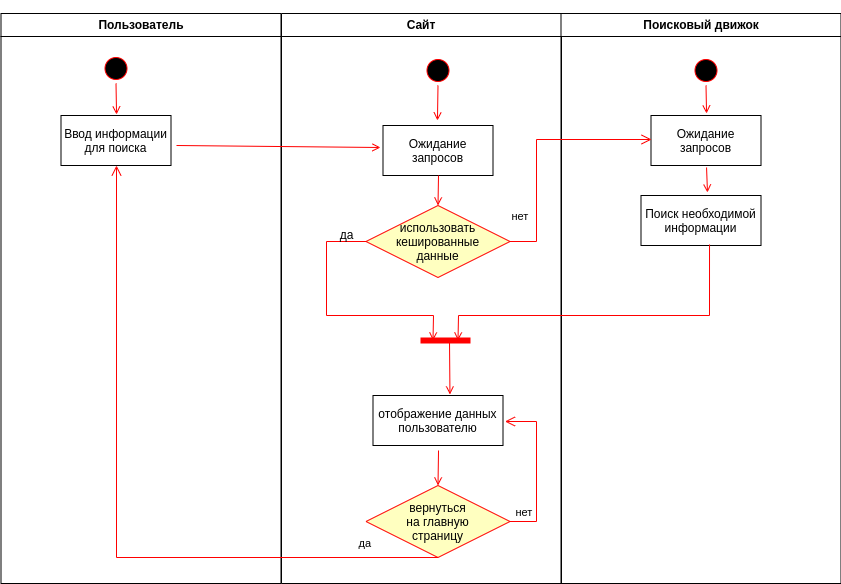
\includegraphics[scale=0.55]{inc/img/activity_diagram.png}
    \caption{Диаграмма активностей для проекта}
\end{figure}

С помощью данной диаграммы можно донести общую концепцию инфраструктуры. Также
на ее основании можно выбрать необходимые для реализации компоненты. Диаграмма
не является точным техническим заданием, а лишь выполняет демонстративную роль.

\section{Архитектура приложения}
\section{Разработка практических решений}
\subsection{Docker}
\subsection{Docker Compose}
\subsection{Scrapy}
\subsection{Scrapyd}
\subsection{Flask}
\subsection{Kafka}
\subsection{Zookeeper}
\subsection{Kafka Connect}
\subsection{Elastic Search}
